\documentclass[12pt,
border=1pt]{standalone}
\usepackage{pgfplots}
\usepackage{amsmath}
\usepackage{amssymb}

\pgfplotsset{compat=newest,
	width=6cm, height=5cm,
	xtick pos=left, ytick pos=left,
	%            scaled x ticks=real:1e-6,
}
% Kernel 2 FP64
\begin{document}
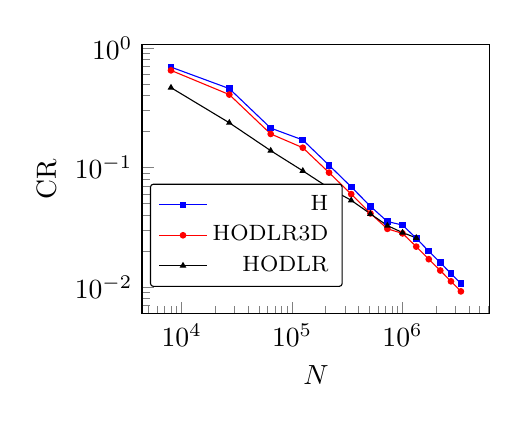
\begin{tikzpicture}[every mark/.append style={mark size=1pt}]
	\begin{axis}[xlabel={$N$},
	ylabel={CR},
%		legend pos=south east,
		legend style={
                at={(0.3,0.1)},
               anchor=south,
               legend columns=1,
               cells={anchor=east},
               font=\footnotesize,
               rounded corners=1pt,
               },
		xmode = log,
	    ymode = log,
	   % xmin = 1e3,
	   % xmax = 1e6,
	   % ymin = 1e-10,
	   % ymax = 1e-0,
	   % xtick={1e-10, 1e-8, 1e-6,  1e-4,  1e-2},
	   % ytick={1e-8, 1e-6,  1e-4,  1e-2, 1e-0}
		]

		%Vaishnavi
		\addplot[
		color=blue,
		mark=square*,
		] coordinates {
(8000,6.944330e-01)
(27000,4.587260e-01)
(64000,2.141660e-01)
(125000,1.704400e-01)
(216000,1.047520e-01)
(343000,6.899990e-02)
(512000,4.741950e-02)
(729000,3.537080e-02)
(1000000,3.303410e-02)
(1331000,2.561130e-02)
(1728000,1.997660e-02)
(2197000,1.601110e-02)
(2744000,1.297700e-02)
(3375000,1.068920e-02)
% (4096000,8.873240e-03)
% (4913000,7.586830e-03)
% (5832000,6.498850e-03)
% (6859000,5.648600e-03)
		};
		%Zhao
		\addplot[
		color=red,
		mark=*,
		] coordinates {
(8000,6.518320e-01)
(27000,4.086830e-01)
(64000,1.914400e-01)
(125000,1.467460e-01)
(216000,9.080690e-02)
(343000,5.999840e-02)
(512000,4.134440e-02)
(729000,3.072430e-02)
(1000000,2.813240e-02)
(1331000,2.180530e-02)
(1728000,1.710820e-02)
(2197000,1.375940e-02)
(2744000,1.116830e-02)
(3375000,9.199400e-03)
		};
		
		\addplot[
		color=black,
		mark=triangle*,
		] coordinates {
(8000,4.672320e-01)
(27000,2.373200e-01)
(64000,1.386470e-01)
(125000,9.395540e-02)
(216000,6.753870e-02)
(343000,5.323050e-02)
(512000,4.102820e-02)
(729000,3.269360e-02)
(1000000,2.859190e-02)
(1331000,2.579220e-02)
		};
		\legend{H, HODLR3D, HODLR}
	\end{axis}
\end{tikzpicture}
\end{document}